

%% bare_jrnl_compsoc.tex
%% V1.4b
%% 2015/08/26
%% by Michael Shell
%% See:
%% http://www.michaelshell.org/
%% for current contact information.
%%
%% This is a skeleton file demonstrating the use of IEEEtran.cls
%% (requires IEEEtran.cls version 1.8b or later) with an IEEE
%% Computer Society journal paper.
%%
%% Support sites:
%% http://www.michaelshell.org/tex/ieeetran/
%% http://www.ctan.org/pkg/ieeetran
%% and
%% http://www.ieee.org/

%%*************************************************************************
%% Legal Notice:
%% This code is offered as-is without any warranty either expressed or
%% implied; without even the implied warranty of MERCHANTABILITY or
%% FITNESS FOR A PARTICULAR PURPOSE! 
%% User assumes all risk.
%% In no event shall the IEEE or any contributor to this code be liable for
%% any damages or losses, including, but not limited to, incidental,
%% consequential, or any other damages, resulting from the use or misuse
%% of any information contained here.
%%
%% All comments are the opinions of their respective authors and are not
%% necessarily endorsed by the IEEE.
%%
%% This work is distributed under the LaTeX Project Public License (LPPL)
%% ( http://www.latex-project.org/ ) version 1.3, and may be freely used,
%% distributed and modified. A copy of the LPPL, version 1.3, is included
%% in the base LaTeX documentation of all distributions of LaTeX released
%% 2003/12/01 or later.
%% Retain all contribution notices and credits.
%% ** Modified files should be clearly indicated as such, including  **
%% ** renaming them and changing author support contact information. **
%%*************************************************************************


% *** Authors should verify (and, if needed, correct) their LaTeX system  ***
% *** with the testflow diagnostic prior to trusting their LaTeX platform ***
% *** with production work. The IEEE's font choices and paper sizes can   ***
% *** trigger bugs that do not appear when using other class files.       ***                          ***
% The testflow support page is at:
% http://www.michaelshell.org/tex/testflow/


\documentclass[10pt,journal,compsoc,onecolumn,draftclsnofoot]{IEEEtran}
%
% If IEEEtran.cls has not been installed into the LaTeX system files,
% manually specify the path to it like:
% \documentclass[10pt,journal,compsoc]{../sty/IEEEtran}





% Some very useful LaTeX packages include:
% (uncomment the ones you want to load)


% *** MISC UTILITY PACKAGES ***
%
%\usepackage{ifpdf}
% Heiko Oberdiek's ifpdf.sty is very useful if you need conditional
% compilation based on whether the output is pdf or dvi.
% usage:
% \ifpdf
%   % pdf code
% \else
%   % dvi code
% \fi
% The latest version of ifpdf.sty can be obtained from:
% http://www.ctan.org/pkg/ifpdf
% Also, note that IEEEtran.cls V1.7 and later provides a builtin
% \ifCLASSINFOpdf conditional that works the same way.
% When switching from latex to pdflatex and vice-versa, the compiler may
% have to be run twice to clear warning/error messages.


\usepackage{graphicx}
\usepackage{listings}



% *** CITATION PACKAGES ***
%
\ifCLASSOPTIONcompsoc
  % IEEE Computer Society needs nocompress option
  % requires cite.sty v4.0 or later (November 2003)
  \usepackage[nocompress]{cite}
\else
  % normal IEEE
  \usepackage{cite}
\fi
% cite.sty was written by Donald Arseneau
% V1.6 and later of IEEEtran pre-defines the format of the cite.sty package
% \cite{} output to follow that of the IEEE. Loading the cite package will
% result in citation numbers being automatically sorted and properly
% "compressed/ranged". e.g., [1], [9], [2], [7], [5], [6] without using
% cite.sty will become [1], [2], [5]--[7], [9] using cite.sty. cite.sty's
% \cite will automatically add leading space, if needed. Use cite.sty's
% noadjust option (cite.sty V3.8 and later) if you want to turn this off
% such as if a citation ever needs to be enclosed in parenthesis.
% cite.sty is already installed on most LaTeX systems. Be sure and use
% version 5.0 (2009-03-20) and later if using hyperref.sty.
% The latest version can be obtained at:
% http://www.ctan.org/pkg/cite
% The documentation is contained in the cite.sty file itself.
%
% Note that some packages require special options to format as the Computer
% Society requires. In particular, Computer Society  papers do not use
% compressed citation ranges as is done in typical IEEE papers
% (e.g., [1]-[4]). Instead, they list every citation separately in order
% (e.g., [1], [2], [3], [4]). To get the latter we need to load the cite
% package with the nocompress option which is supported by cite.sty v4.0
% and later. Note also the use of a CLASSOPTION conditional provided by
% IEEEtran.cls V1.7 and later.





% *** GRAPHICS RELATED PACKAGES ***
%
\ifCLASSINFOpdf
  % \usepackage[pdftex]{graphicx}
  % declare the path(s) where your graphic files are
  % \graphicspath{{../pdf/}{../jpeg/}}
  % and their extensions so you won't have to specify these with
  % every instance of \includegraphics
  % \DeclareGraphicsExtensions{.pdf,.jpeg,.png}
\else
  % or other class option (dvipsone, dvipdf, if not using dvips). graphicx
  % will default to the driver specified in the system graphics.cfg if no
  % driver is specified.
  % \usepackage[dvips]{graphicx}
  % declare the path(s) where your graphic files are
  % \graphicspath{{../eps/}}
  % and their extensions so you won't have to specify these with
  % every instance of \includegraphics
  % \DeclareGraphicsExtensions{.eps}
\fi
% graphicx was written by David Carlisle and Sebastian Rahtz. It is
% required if you want graphics, photos, etc. graphicx.sty is already
% installed on most LaTeX systems. The latest version and documentation
% can be obtained at: 
% http://www.ctan.org/pkg/graphicx
% Another good source of documentation is "Using Imported Graphics in
% LaTeX2e" by Keith Reckdahl which can be found at:
% http://www.ctan.org/pkg/epslatex
%
% latex, and pdflatex in dvi mode, support graphics in encapsulated
% postscript (.eps) format. pdflatex in pdf mode supports graphics
% in .pdf, .jpeg, .png and .mps (metapost) formats. Users should ensure
% that all non-photo figures use a vector format (.eps, .pdf, .mps) and
% not a bitmapped formats (.jpeg, .png). The IEEE frowns on bitmapped formats
% which can result in "jaggedy"/blurry rendering of lines and letters as
% well as large increases in file sizes.
%
% You can find documentation about the pdfTeX application at:
% http://www.tug.org/applications/pdftex






% *** MATH PACKAGES ***
%
%\usepackage{amsmath}
% A popular package from the American Mathematical Society that provides
% many useful and powerful commands for dealing with mathematics.
%
% Note that the amsmath package sets \interdisplaylinepenalty to 10000
% thus preventing page breaks from occurring within multiline equations. Use:
%\interdisplaylinepenalty=2500
% after loading amsmath to restore such page breaks as IEEEtran.cls normally
% does. amsmath.sty is already installed on most LaTeX systems. The latest
% version and documentation can be obtained at:
% http://www.ctan.org/pkg/amsmath





% *** SPECIALIZED LIST PACKAGES ***
%
%\usepackage{algorithmic}
% algorithmic.sty was written by Peter Williams and Rogerio Brito.
% This package provides an algorithmic environment fo describing algorithms.
% You can use the algorithmic environment in-text or within a figure
% environment to provide for a floating algorithm. Do NOT use the algorithm
% floating environment provided by algorithm.sty (by the same authors) or
% algorithm2e.sty (by Christophe Fiorio) as the IEEE does not use dedicated
% algorithm float types and packages that provide these will not provide
% correct IEEE style captions. The latest version and documentation of
% algorithmic.sty can be obtained at:
% http://www.ctan.org/pkg/algorithms
% Also of interest may be the (relatively newer and more customizable)
% algorithmicx.sty package by Szasz Janos:
% http://www.ctan.org/pkg/algorithmicx




% *** ALIGNMENT PACKAGES ***
%
%\usepackage{array}
% Frank Mittelbach's and David Carlisle's array.sty patches and improves
% the standard LaTeX2e array and tabular environments to provide better
% appearance and additional user controls. As the default LaTeX2e table
% generation code is lacking to the point of almost being broken with
% respect to the quality of the end results, all users are strongly
% advised to use an enhanced (at the very least that provided by array.sty)
% set of table tools. array.sty is already installed on most systems. The
% latest version and documentation can be obtained at:
% http://www.ctan.org/pkg/array


% IEEEtran contains the IEEEeqnarray family of commands that can be used to
% generate multiline equations as well as matrices, tables, etc., of high
% quality.




% *** SUBFIGURE PACKAGES ***
%\ifCLASSOPTIONcompsoc
%  \usepackage[caption=false,font=footnotesize,labelfont=sf,textfont=sf]{subfig}
%\else
%  \usepackage[caption=false,font=footnotesize]{subfig}
%\fi
% subfig.sty, written by Steven Douglas Cochran, is the modern replacement
% for subfigure.sty, the latter of which is no longer maintained and is
% incompatible with some LaTeX packages including fixltx2e. However,
% subfig.sty requires and automatically loads Axel Sommerfeldt's caption.sty
% which will override IEEEtran.cls' handling of captions and this will result
% in non-IEEE style figure/table captions. To prevent this problem, be sure
% and invoke subfig.sty's "caption=false" package option (available since
% subfig.sty version 1.3, 2005/06/28) as this is will preserve IEEEtran.cls
% handling of captions.
% Note that the Computer Society format requires a sans serif font rather
% than the serif font used in traditional IEEE formatting and thus the need
% to invoke different subfig.sty package options depending on whether
% compsoc mode has been enabled.
%
% The latest version and documentation of subfig.sty can be obtained at:
% http://www.ctan.org/pkg/subfig



% hyphenation here



\begin{document}
%
% paper title
% Titles are generally capitalized except for words such as a, an, and, as,
% at, but, by, for, in, nor, of, on, or, the, to and up, which are usually
% not capitalized unless they are the first or last word of the title.
% Linebreaks \\ can be used within to get better formatting as desired.
% Do not put math or special symbols in the title.
\title{End of Term Progress Report}
%
%
% author names and IEEE memberships
% note positions of commas and nonbreaking spaces ( ~ ) LaTeX will not break
% a structure at a ~ so this keeps an author's name from being broken across
% two lines.
% use \thanks{} to gain access to the first footnote area
% a separate \thanks must be used for each paragraph as LaTeX2e's \thanks
% was not built to handle multiple paragraphs
%
%
%\IEEEcompsocitemizethanks is a special \thanks that produces the bulleted
% lists the Computer Society journals use for "first footnote" author
% affiliations. Use \IEEEcompsocthanksitem which works much like \item
% for each affiliation group. When not in compsoc mode,
% \IEEEcompsocitemizethanks becomes like \thanks and
% \IEEEcompsocthanksitem becomes a line break with idention. This
% facilitates dual compilation, although admittedly the differences in the
% desired content of \author between the different types of papers makes a
% one-size-fits-all approach a daunting prospect. For instance, compsoc 
% journal papers have the author affiliations above the "Manuscript
% received ..."  text while in non-compsoc journals this is reversed. Sigh.

\author{Tyler Cole, Arnav Bhutani, Team 20}% <-this % stops a space
% note the % following the last \IEEEmembership and also \thanks - 
% these prevent an unwanted space from occurring between the last author name
% and the end of the author line. i.e., if you had this:
% 
% \author{....lastname \thanks{...} \thanks{...} }
%                     ^------------^------------^----Do not want these spaces!
%
% a space would be appended to the last name and could cause every name on that
% line to be shifted left slightly. This is one of those "LaTeX things". For
% instance, "\textbf{A} \textbf{B}" will typeset as "A B" not "AB". To get
% "AB" then you have to do: "\textbf{A}\textbf{B}"
% \thanks is no different in this regard, so shield the last } of each \thanks
% that ends a line with a % and do not let a space in before the next \thanks.
% Spaces after \IEEEmembership other than the last one are OK (and needed) as
% you are supposed to have spaces between the names. For what it is worth,
% this is a minor point as most people would not even notice if the said evil
% space somehow managed to creep in.



% The paper headers
% The only time the second header will appear is for the odd numbered pages
% after the title page when using the twoside option.
% 
% *** Note that you probably will NOT want to include the author's ***
% *** name in the headers of peer review papers.                   ***
% You can use \ifCLASSOPTIONpeerreview for conditional compilation here if
% you desire.



% The publisher's ID mark at the bottom of the page is less important with
% Computer Society journal papers as those publications place the marks
% outside of the main text columns and, therefore, unlike regular IEEE
% journals, the available text space is not reduced by their presence.
% If you want to put a publisher's ID mark on the page you can do it like
% this:
%\IEEEpubid{0000--0000/00\$00.00~\copyright~2015 IEEE}
% or like this to get the Computer Society new two part style.
%\IEEEpubid{\makebox[\columnwidth]{\hfill 0000--0000/00/\$00.00~\copyright~2015 IEEE}%
%\hspace{\columnsep}\makebox[\columnwidth]{Published by the IEEE Computer Society\hfill}}
% Remember, if you use this you must call \IEEEpubidadjcol in the second
% column for its text to clear the IEEEpubid mark (Computer Society jorunal
% papers don't need this extra clearance.)



% use for special paper notices
%\IEEEspecialpapernotice{(Invited Paper)}

% for Computer Society papers, we must declare the abstract and index terms
% PRIOR to the title within the \IEEEtitleabstractindextext IEEEtran
% command as these need to go into the title area created by \maketitle.
% As a general rule, do not put math, special symbols or citations
% in the abstract or keywords.
% make the title area
\maketitle


\begin{abstract}
This document outlines the progress we've made towards our capstone engineering project over the previous term, and what we have left to do. We showcase several of our features and design decisions, changes made  and what we anticipate will be coming over the upcoming term. Furthermore, we include some of the technical snippets and screenshots from our project.
\end{abstract}










% Note that keywords are not normally used for peerreview papers.
\begin{IEEEkeywords}
\centering
Distributed computing, edge network, distributed system, big data, progress report
\end{IEEEkeywords}

\pagebreak 


\IEEEdisplaynontitleabstractindextext

\IEEEpeerreviewmaketitle



\IEEEraisesectionheading{\section{Introduction}\label{sec:introduction}}
\hspace*{-.5cm}The following document outlines the progress made in the construction of a distributed edge computing platform over the last several months. Additionally we will go over some changes plan we plan to make over the remainder of the year. 

\subsection{Purpose}
The purpose of this document is to demonstrate the progress of our big data edge computing platform. It will serve as the primary progress report. 

\subsection{Scope}
This document is primarily a high-level overview of our progress. It is intended to be delivered to a rather technical audience, and pieces of code and screenshots will be included. A large majority of the document can be understood from a non-technical background, however, and much of it can be understood without an extensive technical background.

\section{Progress}
\subsection{Initial Plan}
Our initial plan was crafted very carefully, and we spent quite a bit of time anticipating some of the blockers and issues we might face in the future. Our Gantt chart was meant to illustrate our intended timeline and path to completion for this project. So far, the Gantt chart has done an exceptionally great job at predicting our progress. Our Gantt chart, as created at the near start of the project, can be found below.
    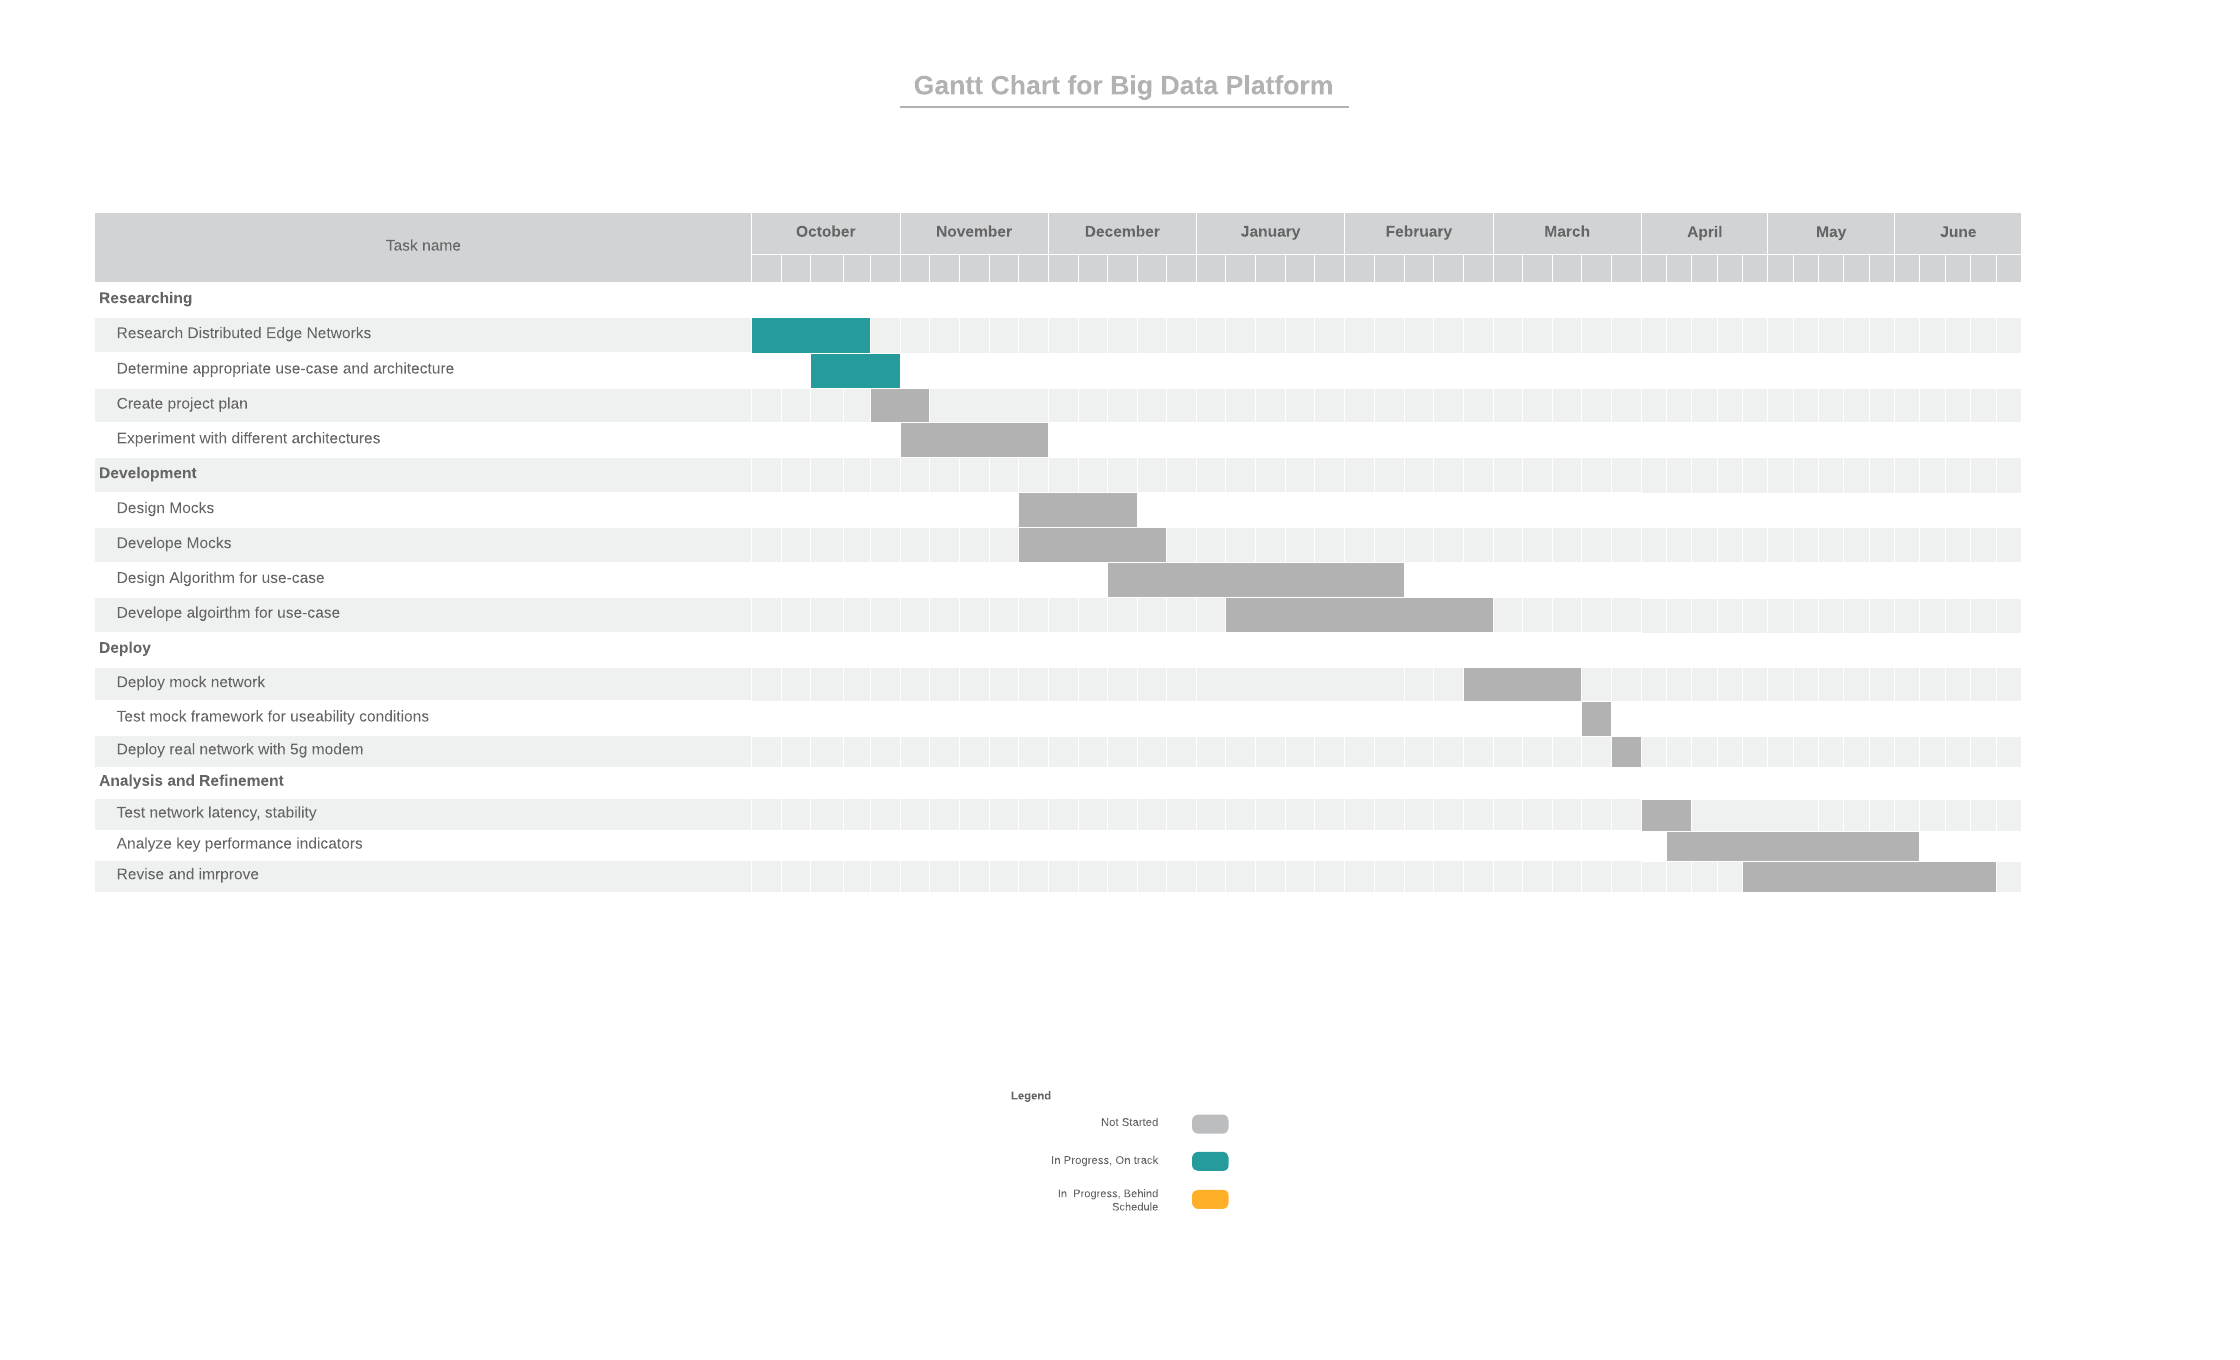
\includegraphics[width=1.10\textwidth]{Gantt.png}
    \hspace*{.5cm}\small{Fig. 1.0. Our Gantt Chart}

As in line with the projections, we are currently still developing the platform on a mock network. That is, although much of the code is completely functional and complete, our application is currently being hosted on a cloud network. Clearly, since our platform is meant to be on the network edge, we still must transfer the platform over to an edge computing device. 

\subsection{Progress} 
Our project progress is split into two sections: Platform Progress, and Application Progress. We're developing a big data, distributed edge computing platform. Our project is meant to both develop a fault tolerant, distributable platform, and also to showcase a potential application on this platform. 
\subsection{Platform Progress}
Our application platform has been developed from scratch, utilizing popular tools such as Docker, Kafka, and Kubernetes to help handle the distribution and configuration of the network. As of today, we have a completely functional distributed edge computing platform, that can be easily configured and scaled horizontally to provide a completely distributed big data platform. The platform architecture is divided into several different stages: data ingestion and preprocessing, stream processing, distribution and computation


\subsubsection{Data Preprocessing}
For data preprocessing We have crafted a custom docker container which is responsible for the preprocessing and data ingestion phase of our application. Although, of course, for any generic application this would have to be expanded upon in order to meet the data preprocessing needs any particular application might require, however the base container for the preprocessing stage is complete. As of now, it reads in image data from the filesystem, and sends that directly to a topic on our kafka message queue.
\subsubsection{Stream Processing}
In order to ensure our system was fault tolerant and easily scalable, we needed to tunnel our data through a message queue to be able to reliably process high volumes. Kafka and Zookeeper were decided upon to do this. We developed two kubernetes manifest files, one to initialize a zookeeper deployment and service, and another to initialize our kafka queue and a service such that it could be connected to from within the network. 
\subsubsection{Distribution}
Every component of our platform has been engineered such that it can be horizontally scaled automatically. We chose to use kubernetes deployments, such that any particular container can be rolled out continuously, without even encountering any downtime in the service. Since each of our containers were engineered from public docker containers, and are available onliny, any application can copy and work directly from our docker images in order to further customize any particular component of our system.
\subsubsection{Computation}
As of now our computation containers read directly from the kafka message queue and process the images directly. There can be any number of computation containers running at any given instance, and they can process the data in parallel. Our example application is an excellent instance of this, where there is three computation containers simultaneously processing data from a single input. 

\subsection{Application Progress}
To showcase our distributed computing platform, we integrated an extremely powerful machine learning algorithm known as YOLO, into our computation containers. Although, our platform is meant to be a generic big data computing platform, therefore an analogous result could be demonstrated with hypothetically any machine learning algorithm. 

\subsubsection{Application}
Our implementation of the YOLO algorithm is fully functional and succinctly demonstrates the functionality of our platform. As of now, we are not actually doing anything with the YOLO output rather than displaying it, as that's not the primary focus of our application. In a practical setting, however, the output would likely be tunneled back to the local client or up to a cloud provider such that the results could be processed in a large data warehouse.

\section{Problems}
\subsection{Lack of Physical Computer}
As of now, by far the largest limitation of our application is the lack of a physical device to develop our edge computing platform on. That is, our \textit{edge} computing platform is currently be developed in the cloud. This is clearly problematic, and is a seriously large blocker but that we're currently unable to get past. Although we can most certainly continue development of our application on the cloud, we will not be able to begin configuring or fine-tuning the system on the network edge until we have received this device. \\
\hspace*{.5cm}\\
Our client, Rahul, is going to provide us with single board computers that we can use to deploy the edge network on. Ideally, we will have a multitude of devices that are 5g connected and can communicate and collaborate seamlessly without any regard to the particular hardware the pod is running on. There will be differences as to how our cloud is currently set up, but for now we can only try our best to anticipate the problems we might run in to. 

\subsection{Limitations of Kafka-Python}
Another large problem we've ran into is the limitations of having Kafka as the intermediary between the ingestion phase and the computation phase. Although Kafka is an extremely reliable and robust platform, it still has its limitations. Unfortunately, Kafka is supported on Java for the most part, and doesn't have a lot of portability to other langauges. We've managed to integrate a library in python which reads from our Kafka queue, because python is one of the most popular machine learning algorithms, however this would likely extend to other more obscure langauges. 

\section{Plans}
\subsection{Network edge}
We still need to move the platform to the edge of the network, which we anticipate to be quite challenging. This will largely consist of setting up the devices, and connecting them to a portable 5g modem and configuring them to be able to talk to each other over the cluster network. This, although sounds rather straightforward, can be extremely difficult to set up correctly such that our platform could be initialized on any set of 5g capable devices and be deployed easily. 

\subsection{Spark big data}
Our platform is currently reading data directly from Kafka and using standard input to process the data. This is an adequate solution, however the Spark streaming framework has a slew of tools and capabilities that would boost efficiency, and provide an extremely easy to use programming interface. This is one of our stretch goals for the project, however we are certainly planning to get it integrated because of the variety of benefits it would provide to clients developing on the platform.

\subsection{Tunnel through filesystem}
Although in many cases, our network would require TCP communication between nodes, there are also cases when the node running the kafka container would also be the node running the processing containers. Therefore, if we could bypass the intra-network communication and pass the data directly through the filesystem of the node itself, that would drastically reduce the overhead for transferring data and make our system exponentially more efficient. This would be quite a challenge to complete, however we plan to conduct more research into the possibility of this and hopefully implement it into our platform. 


\section{Demonstration}
\subsubsection{Network Architecture}
As previously described, our network architecture is strictly divided into a couple key isolated components running in kubernetes deployments and services. Below is a screenshot of the totality of our platform architecture given through kubernetes. 
\begin{center}
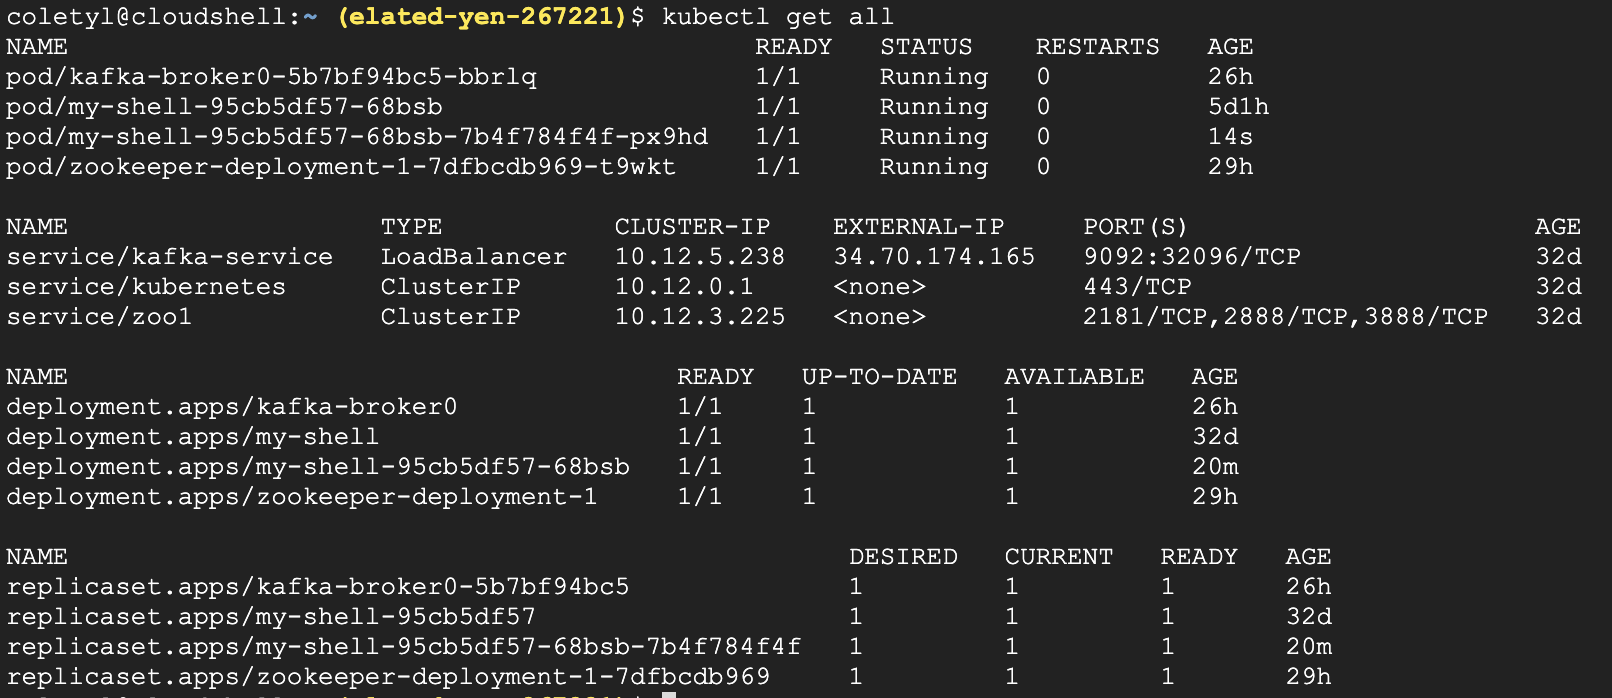
\includegraphics[width=.95\textwidth]{kube-output.png}\\
\end{center}
\hspace*{.5cm}\small{Fig. 2.0. Output of byte-stream encoding of video from kafka}



\subsubsection{Kafka and Zookeeper}
The Kafka and Zookeeper components consist of a kubernetes deployment and service. The deployment is the generic container that the zookeeper and kubernetes applications actually run on, and the service exposes their endpoints so they can be accessed from within the network. Below is the kubernetes manifest of the zookeeper deployment and service as well as a screenshot of the kafka listings be accessed from the command line
\begin{lstlisting}
kind: Deployment
apiVersion: extensions/v1beta1
metadata:
  name: zookeeper-deployment-1
spec:
  template:
    metadata:
      labels:
        app: zookeeper-1
    spec:
      containers:
      - name: zoo1
        image: digitalwonderland/zookeeper
        ports:
        - containerPort: 2181
        env:
        - name: ZOOKEEPER_ID
          value: "1"
        - name: ZOOKEEPER_SERVER_1
          value: zoo1
---
apiVersion: v1
kind: Service
metadata:
  name: zoo1
  labels:
    app: zookeeper-1
spec:
  ports:
  - name: client
    port: 2181
    protocol: TCP
  - name: follower
    port: 2888
    protocol: TCP
  - name: leader
    port: 3888
    protocol: TCP
  selector:
    app: zookeeper-1
\end{lstlisting}
\hspace*{.5cm}\small{Fig. 3.0. The Zookeeper deployment and service manifest}
\begin{center}
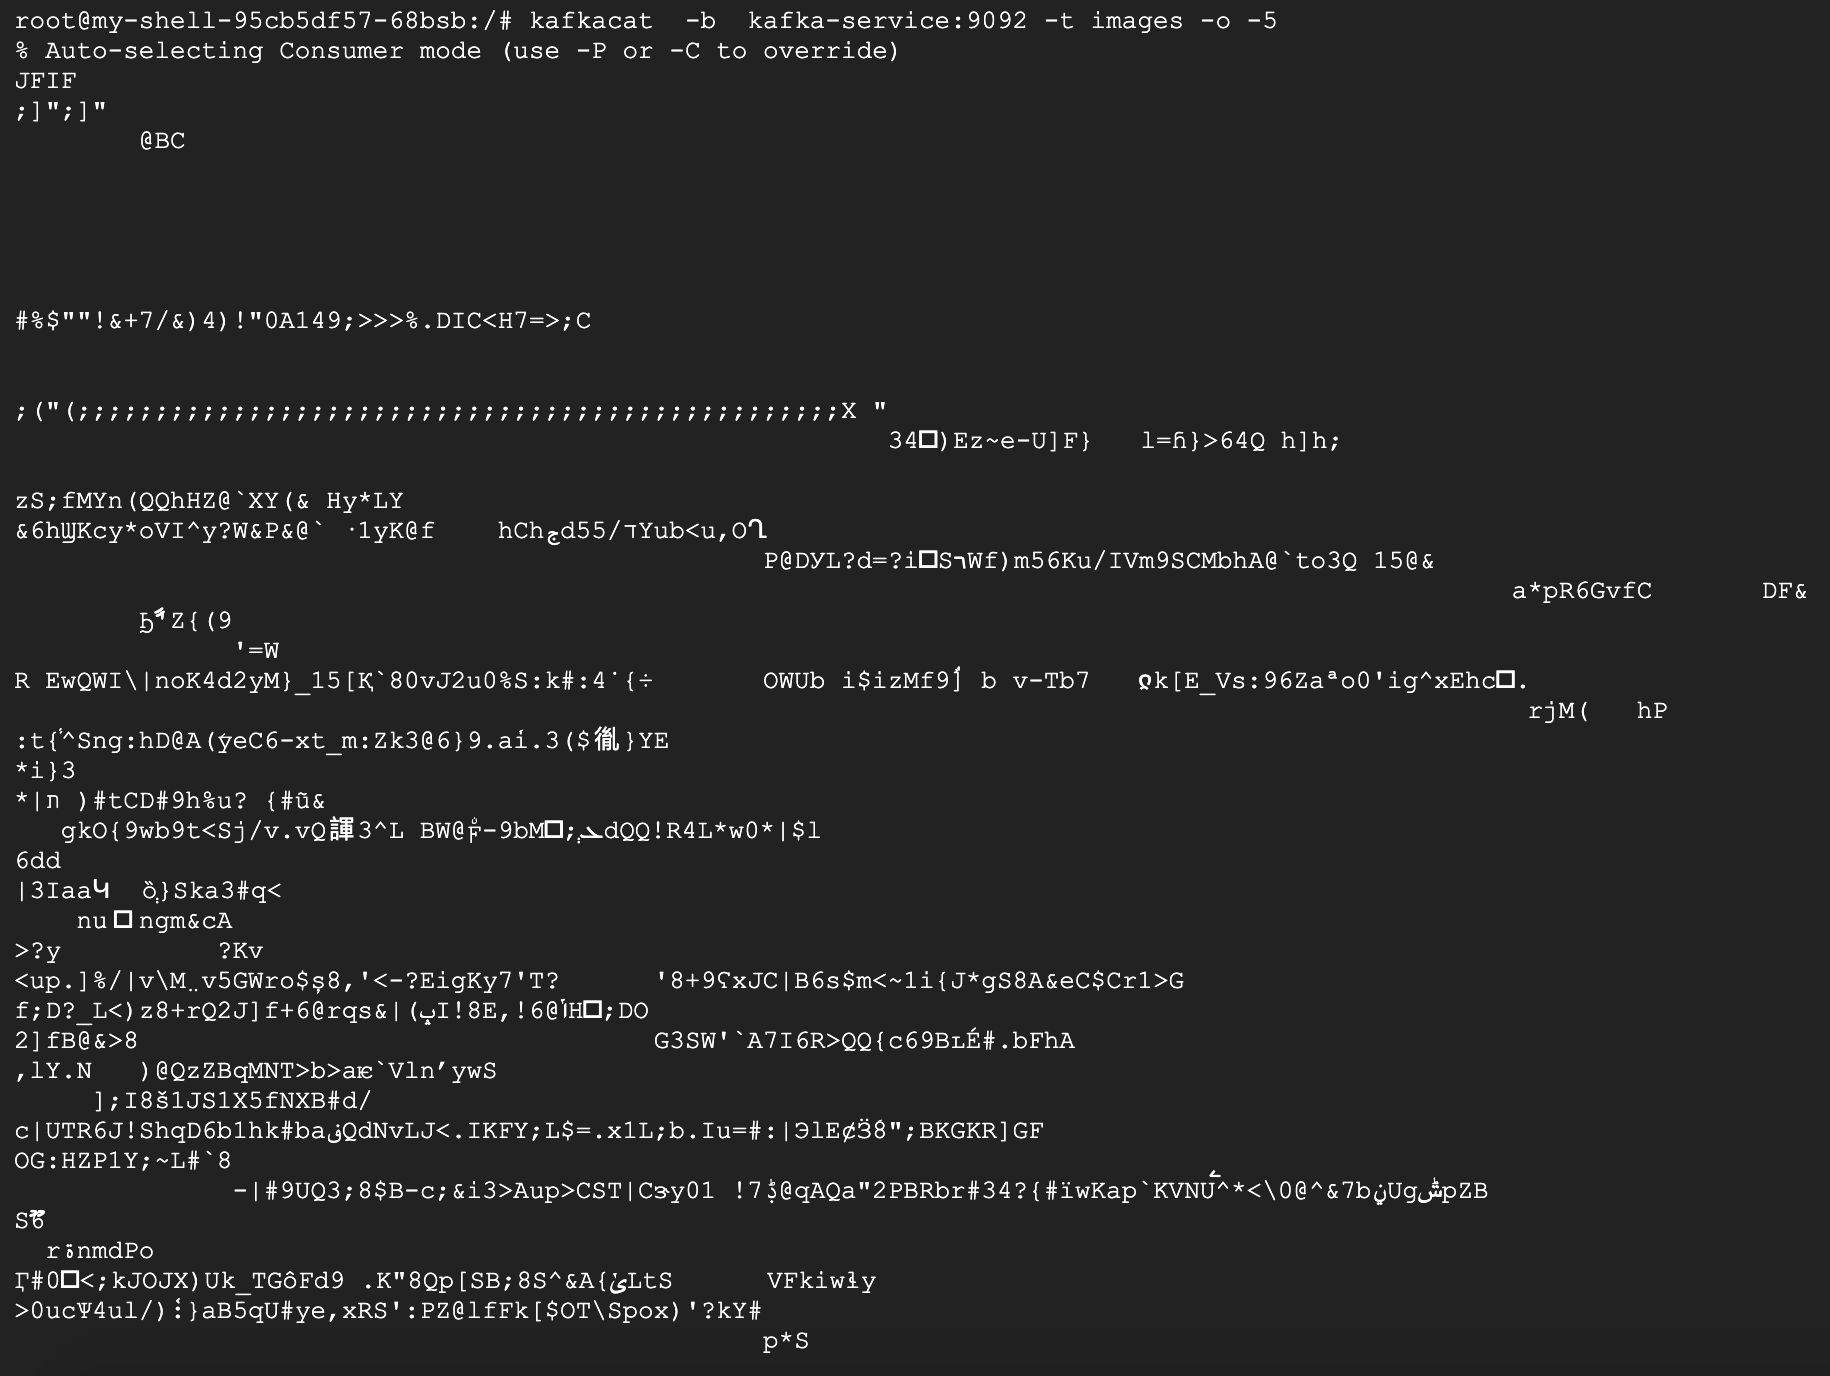
\includegraphics[width=.95\textwidth]{kafka-output.png}\\
\end{center}
\hspace*{.5cm}\small{Fig. 4.0. Output of byte-stream encoding of video from kafka}

\subsubsection{YOLO Algorithm}
The Yolo container is made up of two parts: the kafka consumer and the yolo algorithm. The consumer is connected to the Kafka Broker pod on the services' exposed port. The consumer requests a single image from the broker and then caches the result of that request. The cache is then classified by the Yolo algorithm and the output is then printed to stdout, which can be accessed by the logging algorithm.\\
\linebreak
\newline
Below is the kubernetes manifest of the yolo application:
\begin{lstlisting}
apiVersion: apps/v1
kind: Deployment
metadata:
  name: yolo-deployment
  labels:
    app: yolo
spec:
  replicas: 1
  selector:
    matchLabels:
      app: yolo
  template:
    metadata:
      labels:
        app: yolo
    spec:
      containers:
      - name: yolo-container
        image: bhutaniarnav/yolo-docker-2:latest
        env:
        - name: KAFKA_HOST_NAME
          value: "kafka-service"
        ports:
        - containerPort: 80

\end{lstlisting}
\hspace*{.5cm}\small{Fig. 5.0. The Yolo Container's Kubernetes manifest}\\
\linebreak
\newline
Below is the dockerfile for the yolo-container:
\begin{lstlisting}
FROM ubuntu:18.04
LABEL maintianer="Arnav Bhutani"

ENV DEBIAN_FRONTEND noninteractive

ARG ADDITIONAL_PACKAGES="python3.6 python3-pip libopencv-dev wget"

RUN apt-get update \
      && apt-get install --no-install-recommends --no-install-suggests -y gnupg2 ca-certificates \
            git build-essential $ADDITIONAL_PACKAGES \
      && rm -rf /var/lib/apt/lists/*

COPY ./configure.sh /tmp/
COPY ./startup.sh /tmp/

RUN pip3 install kafka-python
RUN wget https://pjreddie.com/media/files/yolov3.weights

ARG SOURCE_BRANCH="master"
ARG SOURCE_COMMIT="d51d89053afc4b7f50a30ace7b2fcf1b2ddd7598"
ENV SOURCE_BRANCH $SOURCE_BRANCH
ENV SOURCE_COMMIT $SOURCE_COMMIT

ARG CONFIG

RUN git clone https://github.com/AlexeyAB/darknet.git && cd darknet \
      && git checkout $SOURCE_BRANCH \
      && git reset --hard $SOURCE_COMMIT \
      && /tmp/configure.sh cpu-cv && make \
      && cp darknet /usr/local/bin \
      && cp -r cfg / \
      && cp -r data / \
      && cd .. && rm -rf darknet

RUN git clone https://github.com/Involution124/BigData.git && cd BigData/DockerPythonConsumer \
      && cp app.py / \
      && cd ../.. && rm -rf BigData

CMD ["python3", "-m",  "app"]
\end{lstlisting}
\hspace*{.5cm}\small{Fig. 6.0: The Yolo Container's Docker file}\\
\linebreak
\newline
Below is the output from the yolo container:
\begin{center}
    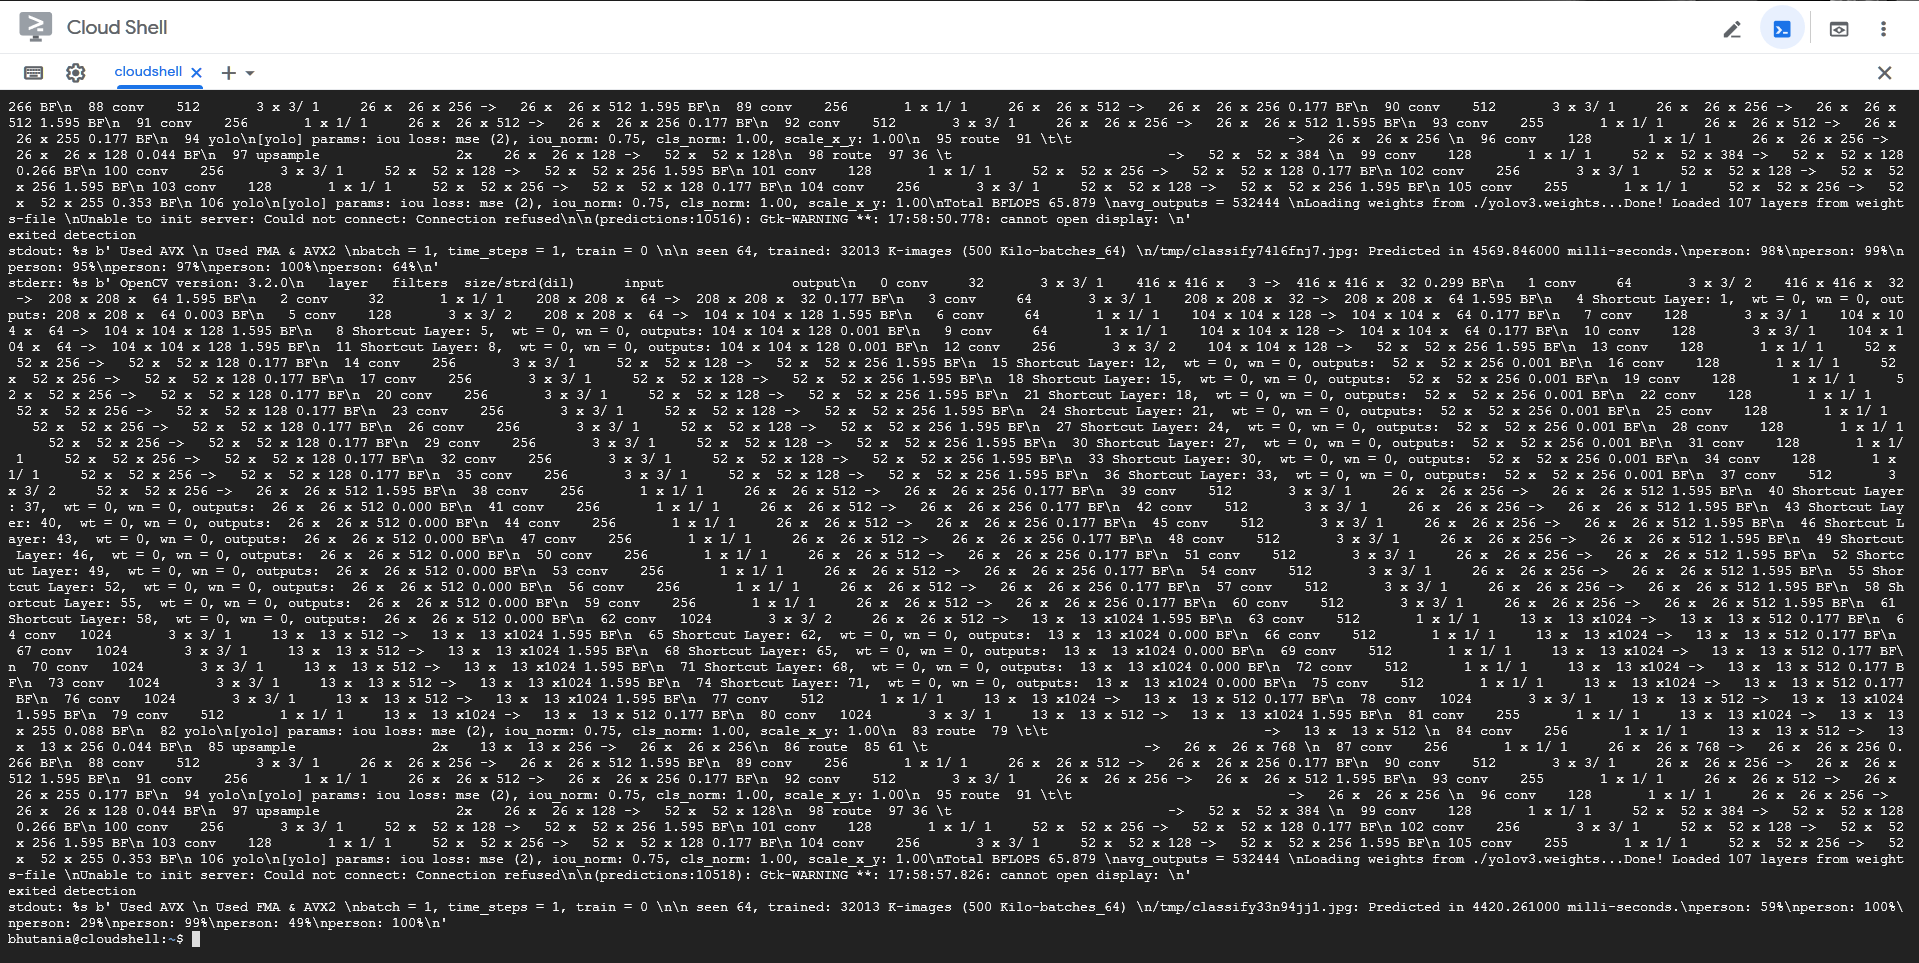
\includegraphics[width=.95\textwidth]{yolo.png}
\end{center}

\hspace*{.5cm}\small{Fig. 7.0. The Yolo Container's output}\\



\subsection

\end{document}


